\chapter{Wireless propagation models}\label{ch:channelmodellingbasics}

The propagation of waves in any medium can be modeled using fundamental principles of physics. It has been shown that the fundamental understanding of these physics are quite accurate and can provide any researcher with a satisfactory knowledge of how waves propagate in air. Wireless transmission is essentially electromagnetic radiation from a transmitter to a receiver. We have the well known \emph{Maxwell} equations for calculating the electromagnetic fields that is received. From such equations it can be seen that as distance $r$ increases the electric field decreases with $r^{-1}$. This means the power of the field decreases by $r^{-2}$ given a sphere is radiating. This is only if we assume the surface area of such a sphere increase as $r^2$ \cite{Tse2005FundamentalsCommunication}. Such a notion is only relevant in free space propagation situation where no reflections are happening, which in the world of mobile communication systems is not typical. Even a very simple situation (such as a reflecting wall and a moving antenna) can be shown to significantly change the profile of the electromagnetic field and its power. This is due to patterns of constructive and destructive interference. This is also known as multipath fading, thus signals can propagate along different paths but arrive at the same time cancel (effectively) each other out. In practice many obstacles are present in a transmission scenario, which means that the power at the receiver decreases with distance much faster than $r^{-2}$. At large distances such a decay is exponential-like. The modelling of this decay in practical transmission scenarios (and the nature of it) is the purpose of this chapter.

Obstacles in the transmission scenario cause signal attenuation as power is absorbed and scattered. This phenomenon is known as shadowing, and can be seen as obstacles blocking (or partly block) the dominant paths of the traversing radio waves. The attenuation of a signal is thus varying over time and frequency, but also determined largely by the obstacles in the radio environment. This complex function of attenuation is normally and regularly described using two key terms, \emph{slow} and \emph{fast} fading. Also termed, Large-scale or Small-scale fading respectively. Both have been studied extensively and can be modeled using statistical and geometric principles.

\paragraph{Large-scale fading}
also known as \emph{slow} fading, is the product of obstacles shadowing the signal. This can also be seen as a change in the number of scatters for a receiver in a given position $x,y,z$. In other words, such obstacles change the paths and reflections of the radio waves which cause spatially determined fluctuations of attenuation at the receiver. 


\paragraph{Small-scale fading}\label{sec:small_scale_fading}
also known as \emph{fast} fading, or just \emph{fading} \cite{Rappaport:2001:WCP:559977} is the effect of interference between several verions of the transmitted wave arriving shifted in time. This is caused by obstacles in the propagation environment causing reflections thus the waves arrive from many directions and with different propagation delays. A large quantity of factors influence small-scale fading such as multipath propagation, the speed of the mobile, the speed of surrounding objects and the bandwidth of the signal. A comprehensive description of small-scale fading can be found in \cite{Rappaport:2001:WCP:559977}. 


\section{Established methodologies for received power estimation}
The received power is determined not only by the impairments and path losses associated with the wireless channel. Several other items have an impact on the final received power. Modelling the final received power is commonly done through the use of so-called link budgets. The link budget is an essential part of designing reliable communication systems and can give insights in the needed requirements of the hardware composing the communication system \cite{Molisch2007}.


\begin{equation}\label{eq:link_budget}
    P_{rx} = P_{tx} + G_{tx} - L_{tx} - L_{PL} + G_{rx} - L_{rx}
\end{equation}

Here $P_{rx}$ is the received power, $P_{tx}$ is the transmitted power, $G_{tx}$ and $L_{tx}$ are gains and losses associated with the transmitter. $G_{rx}$ and $L_{rx}$ are gains and losses associated with the receiver and finally, $L_{PL}$ are the path losses. The complete estimation of received power consists thus of a multitude of terms. In most cases gains and losses of both the receiver and transmitter components can be quite accurately approximated through calibration procedures  \cite{Molisch2007}. The above link budget is rather simplified for use in mobile communication systems and should contain many more parameters to accurately predict received power. In any case the most attenuation of the link budget is associated to path losses, thus predicting and estimating accurate path losses is the most essential element. Unfortunately the task of estimating accurate path losses are either 1) computational complex to ensure high accuracy or 2) computational fast but at the cost of inaccurate estimations. Models for obtaining path loss estimations are from hereon termed \emph{wireless channel models} or just \emph{channel models}. However, it is important to note that wireless channel models must consider not only power but also delays and other components. A complete overview of wireless channel models will not be given in this dissertation, and the reader is refereed to the content of common textbooks such as \cite{Tse2005FundamentalsCommunication}.

Obtaining approximations of $L_{PL}$ is challenging and many approaches for doing so have been developed over the existence of mobile communication systems. Channel models for wireless transmission have been subject to much research and are seperated into two fundamental \emph{families} of channel models. Such families are either considered \textbf{statistical} or \textbf{geometric}. This chapter will outline the purpose and properties of various existing channel modelling methodologies. This is necessary in order to motivate and visualize where learning methods could improve the current methodologies.

\begin{figure}[thbp]
    \centering
    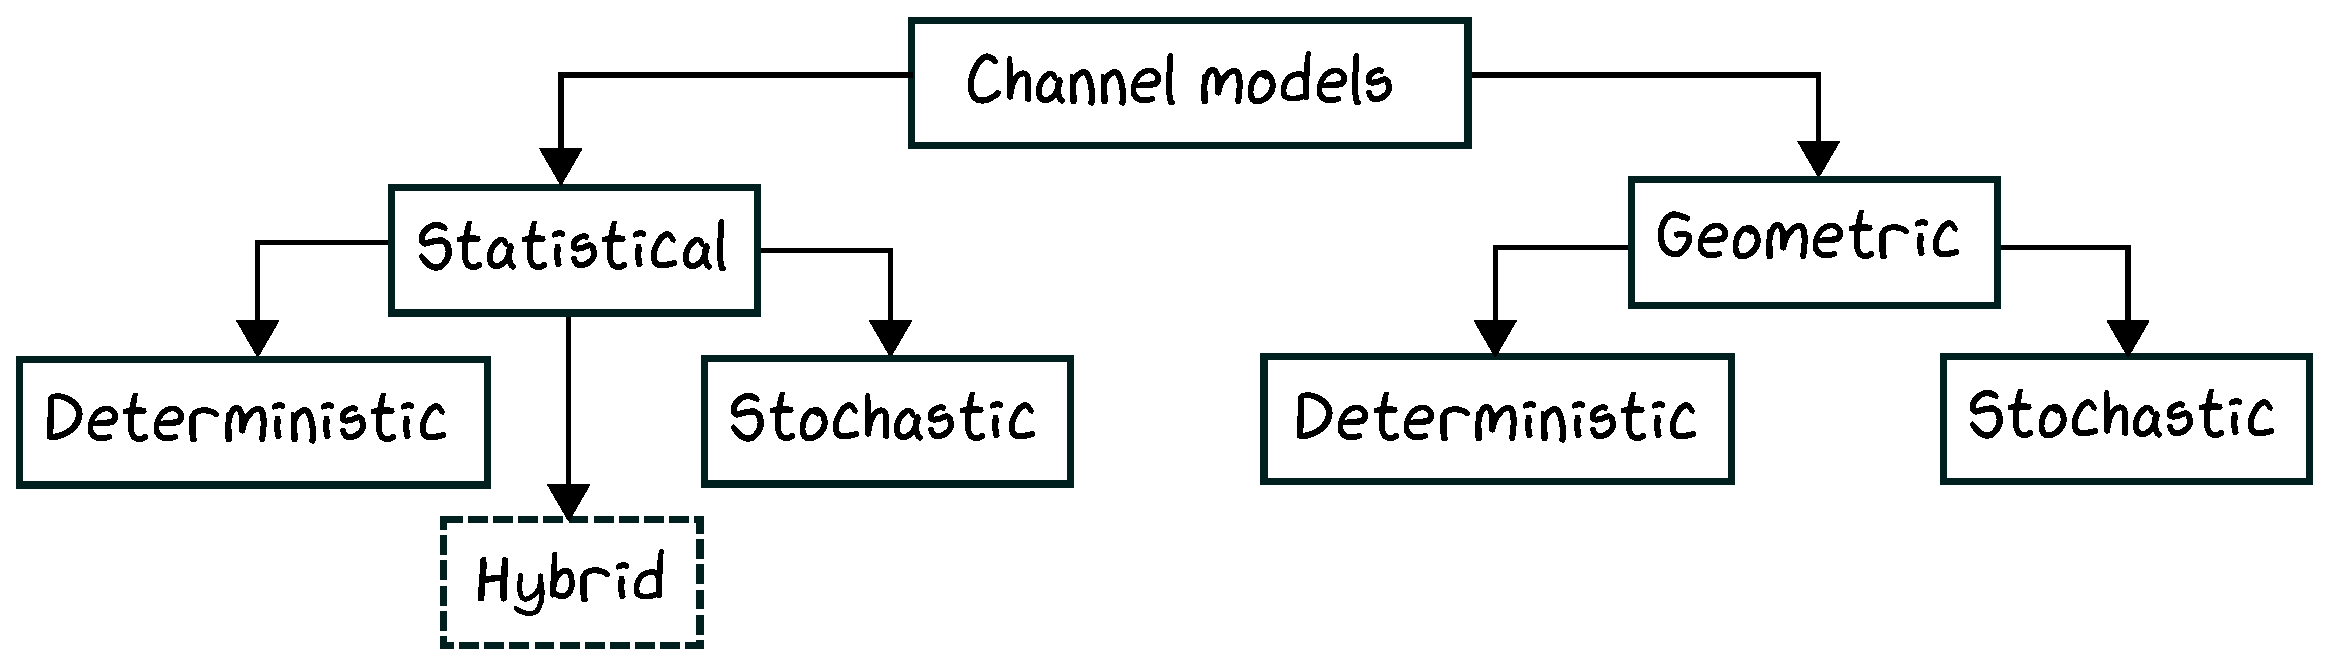
\includegraphics[width=\textwidth]{chapters/part_pathloss/figures/channelmodel_tree.eps}
    \caption{Two \emph{families} of channel models have been the default approach for modelling the wireless transmission impairments. Each of the families, statistical and geometric deal with both deterministic and stochastic approaches. Recently hybrid methods have gained attention for improving accuracy while keeping valuable statistical properties.}
    \label{fig:channel_models}
\end{figure}


\subsection{Statistical}
By obtaining measurements of radio propagation, the resulting statistics can be studied and exploited for estimating path loss. This is the basis of so-called \emph{statistical channel models}, also termed \emph{empirical models}. The use of statistical methods have a long standing history due to the simplistic required analysis. The variations of path loss can furthermore be described with additional statistics in a stochastic setting. For instance, the variations provided by large-scale fading impairments have been found to be representative with a log-normal distribution. The parameters of the distribution is then propagation scenario dependent. Additional approaching for utilizing such statistics can be found in Section \ref{sec:stochastic_channel_model}.

Analysing the statistics of radio propagation measurements is a practical way of obtaining effective approximations of the radio channel. However, it can also be understood that engineering statistics to cover all possible transmission scenarios is simply not feasible. For such reasons the statistical methods turn to stochastic approaches which can offer valuable margins for further link budget analysis. In some well defined propagation scenarios a set of deterministic features enable increased accuracy in path loss estimation which have sparked hybrid models. These hybrid models mix very specific propagation statistics with a stochastic representation of any variations in the path loss. 

Statistical methods is a classical way of providing path loss estimations using regression techniques. A brief introduction to such models can be found in Section \ref{sec:empirical_path_loss}.


\subsection{Geometric}
In practice radio propagation can be described as the propagation of \emph{radiowaves} through electromagnetic radiation. This can in a theoretical and mathematical setting be reduced to the idea of the waves taking certain \emph{paths} determined by the objects in the propagation environment. Geometric models is the study and thus approximation of how the radiating radiowaves will propagate throughout the given propagation scenario. This is reduced to computing the most dominant and likely paths the signal will traverse \cite{Tse2005FundamentalsCommunication}. In essence the result of doing so is in principle an approximate solution to utilizing Maxwell's equations. Geometric channel models are based on these principles and can be reduced to a deterministic and stochastic representation.

Ray-tracing is a deterministic way of computing the dominant and likely paths in a propagation scenario by assuming a finite number of reflectors. However, such channel models require detailed information of objects present in the propagation environment, which can be a significant bottleneck in the creation of such models. Example of ray-tracing models and the resulting accuracy are given in Section \ref{sec:ray-tracing}.

Geometric stochastic models consists of representing so-called \emph{scatterers} in the radio environment by using not only distributions of spatial location, but also the distributions of the resulting angle of propagation. Such models are essential for the study and simulation of realistic \gls{mimo} transmission.  

\section{Empirical path loss models}\label{sec:empirical_path_loss}

One of the earliest examples of such a model is the Free-space path loss model \cite{Goldsmith2005WirelessCommunications}. However, as noted earlier models assuming free-space struggle in outdoor propagation scenario with the presence of many objects and the resulting obstruction of transmission. One of the earliest examples of a path loss model derived and calibrated for urban propagation statistics is the Okumuara-Hata propagation path loss model \cite{Hata1980}. The authors showed that a model with simple parameters is capable of predicting path loss with satisfactory accuracy using a function of distance. The field strength can be described as a function of distance ($R$) following the form
\begin{equation}
    L(dB) = A + B \log_{10} R
\end{equation}

\begin{marginfigure}
    \centering
    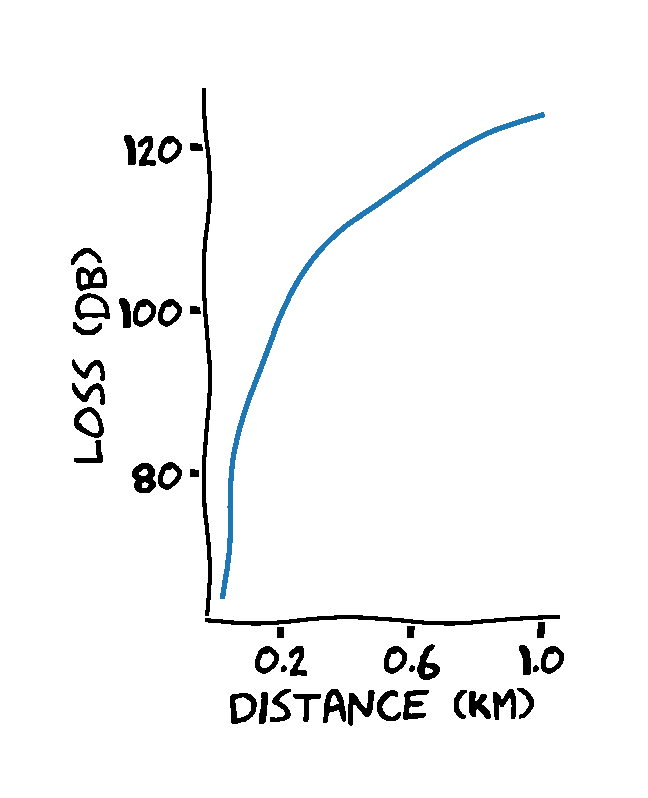
\includegraphics{chapters/part_pathloss/figures/okumura-hata-pathloss.eps}
    \caption{The Okumuara-Hata path loss model and the exponential decay of attenuation related to distance.}
    \label{fig:my_label}
\end{marginfigure}

Where $A$ and $B$ are correction factors that account for characteristics of the propagation scenario, such as the transmitter/receiver antenna height and the frequency. Such parameters, $A$ and $B$ was derived using field measurements in an attempt to \emph{generalize} the propagation characteristics. It has ever since been validated to be a simple and effective approach of estimating losses related to distance of transmission. A few corrections to the original models have been made over the years which has resulted in new measurement studies. These studies have paved the way for more accurate path loss models that is capable of generalizing more propagation scenarios.

Significant efforts have been spent in an attempt to achieve empirical path loss models that generalize well. This is illustrated by the recent technical documents as proposed by \gls{3gpp} and \gls{itu}. In particular, the documents of interest are titled

\begin{itemize}
\item \textbf{\gls{3gpp} TR 38.901 - \cite{3GPP38901}} - Study on channel model for frequencies from 0.5 to 100 GHz
\item \textbf{\gls{itu}-R M.2412 \cite{ITU2412}} - Guidelines for evaluation of radio interface technologies for IMT-2020
\end{itemize}

In both sources a detailed process for the modelling for radio propagation for mobile communication networks is supplied and summarized. The content of both documents are thus considered the default approach for modelling the wireless channel in mobile communication systems per \gls{lte} and \gls{nr} deployed solutions. The content of both documents are rather vast, a focus on the modelling of mean path loss using the empirical models under shadow-fading impairments are given below.

\subsection{Propagation scenarios under consideration}
Inherently different settings of propagation. An attempt to generalize the amount of obstacles and overall propagation characteristics of a given propagation scenario. For example, as defined by \gls{3gpp} in \emph{38.901} are three distict propagation scenarios, each considering different statistics. 

\begin{itemize}
    \item \gls{rma}
    \item \gls{uma}
    \item \gls{umi}
\end{itemize}

For the case of ITU-R M.2412 \cite{ITU2412} a few additions are given. Moreover, such additions are defined as \emph{test environments} for IMT-2020 and are as follows
\begin{itemize}
    \item Indoor-\gls{embb}
    \item Dense Urban-\gls{embb}
    \item Rural-Indoor-\gls{embb}
    \item Urban Macro-\gls{mmtc}
    \item Urban Macro-\gls{urllc}
\end{itemize}

Such environments does not only define a path loss models, but also more specific transmission configuration parameters along with more general network configuration parameters. For example, each of the listed test environments consider specific configurations of \gls{ue} density. A large selection of configuration details for each of the test environments can be found in \cite{ITU2412}.


The title of the \gls{3gpp} document makes the point quite clear. Having channel models that are capable of generalizing losses in the frequency range of 0.5 to 100 GHz. A complication of state of the art measurements campaigns have been utilized in both documents, and the share many similarities. Without summarizing the entirety of the documents, the main differences (in terms of path loss models) can be outlined as:

\begin{itemize}
\item M.2412 offers:
\begin{itemize}
\item \gls{inh}\_A, \gls{inh}\_B
\item Dense urban: \gls{uma}\_A, \gls{uma}\_B, \gls{umi}\_A, \gls{umi}\_B
\item Rural: \gls{rma}\_A, \gls{rma}\_B
\end{itemize}
\item \gls{3gpp} 38.901
\begin{itemize}
    \item Indoor: \gls{inh}
    \item Urban: \gls{uma}, \gls{umi}
    \item Rural: \gls{rma}
\end{itemize}
\end{itemize}

Thus, M.2412 offers models termed $A$ and $B$. The difference is related to the carrier frequency ($f_c$). Models termed $A$ is for a frequency range of $0.5\; \text{GHz} \leq f_c \leq 6 \;\text{GHz}$. Whereas $B$ is for $0.5 \; \text{GHz} \leq f_c \leq 100 \; \text{GHz}$. In relation to 3GPP TR 38.901 this is slightly different. The ITU model termed $B$ is identical (and based on the same channel measurement campaigns) to that of 3GPP 38.901. A \gls{los} and \gls{nlos} model exist for all propagation scenarios. The modelling of the \gls{los} state is similar for both documents and is briefly outlined in section \ref{subsec:los}.

\subsection{Recent empirical path loss models}

In \gls{3gpp} TR 38.901, attenuation for an Urban Macro scenario (\gls{uma}), given a \gls{nlos} transmission state is defined as

\begin{equation}\label{eq:uma_nlos_pathloss_max}
     PL_{UMa-NLOS}^{'} = \text{max} \left( PL_{UMa-LOS}, PL_{UMa-NLOS}^{'} \right)
\end{equation}

Where

\begin{align}\label{eq:uma_nlos_pathloss}
\begin{split}
     PL_{UMa-NLOS}^{'} &= 13.54+39.08\log_{10}(d_{3D}) \\
      &\quad+ 20\log_{10}(f_c) - 0.6(h_{UT}-1.5) \\
  \end{split}
 \end{align}

Additionally, it uses the \gls{uma} \gls{los} model, $PL_{UMa-LOS}$. The loss in the \gls{los} model is dependent on a so-called \emph{breakpoint} distance which essentially turns the path loss function into to a multistep path loss function. The breakpoint distance is defined as $d_{bp} = 4 h_{BS} h_{UT} f_c / c$. In summary, the empirical model is a factor of the following parameters: $\mathbf{h_{BS}}$ (Base station height), $\mathbf{h_{UT}}$ (User terminal height), $\mathbf{d_{3D}}$ ($3$D distance), and $\mathbf{f_c}$ (Carrier frequency). The \gls{3gpp} path loss models can be found in \cite{3GPP38901} Table 7.4.1-1. 

The \gls{rma} model utilize additional parameters of $\mathbf{h}$ (average building height) and $\mathbf{W}$ (average street width).

% \begin{align}\label{eq:rma_nlos_pathloss}
% \begin{split}
%     PL_{RMa-NLOS} &= 161.04-7.1\log 10( W) + 7.5 \log 10(h) \\
%      &\quad- (24.37 -3.7*(h/h_{bs})^2)\log 10(h_{bs}) \\
%      &\quad+(43.42 - 3.1\log 10(h_{bs}))(\log 10(d_{3D})-3) \\
%      &\quad+20\log 10(f_c) - (3.2(\log 10(11.75h_{UT}))^2 - 4.97)
%  \end{split}
% \end{align}

\subsection{Stochastic modelling of impairments}\label{sec:stochastic_channel_model}
The complete budget of attenuation related to transmission can be modeled as a \emph{\textbf{statistical and stochastic process}} by introducing terms for fading. More specifically, terms for Large-scale fading and Small-scale fading. Parameters related to these phenomenons are termed \gls{lsp} and \gls{ssp} respectively. It has been shown that the overall loss can be modeled as described

\begin{equation}\label{eq:pathloss_model}
  PL(d,t) = L(d) + X_\sigma + L(t)
\end{equation}

Where $L(d)$ is the mean path loss, for instance the \gls{uma} model as seen in Eq. (\ref{eq:uma_nlos_pathloss_max}), $X_\sigma$ is shadow fading and $L(t)$ is small-scale fading. Guidelines and parameters of both the large- and small-scale terms are given in the \gls{3gpp} and \gls{itu} documents. The amount of parameters are quite significant thus only a small selection of principles, methodologies and parameters are included in this dissertation. 

\begin{figure}
    \centering
    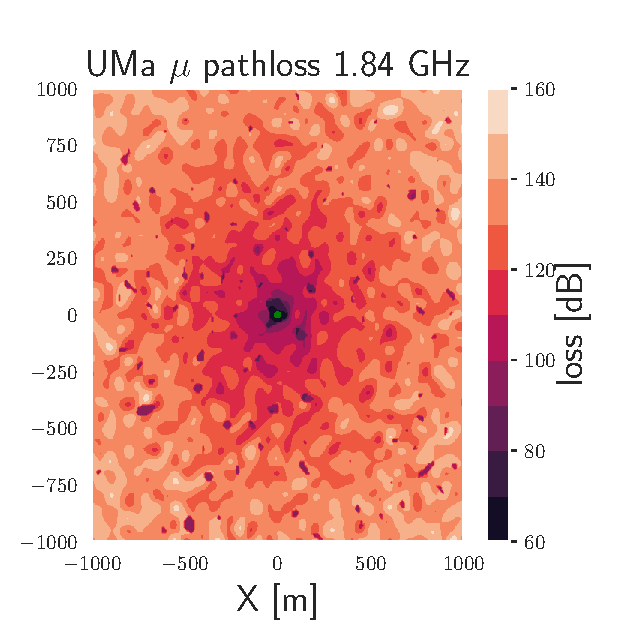
\includegraphics[width=0.6\textwidth]{chapters/part_pathloss/figures/UMaPL.eps}
    \caption{Example of Eq. (\ref{eq:pathloss_model}) for a time-invartiant channel with spatial consistency.}
\end{figure}


\subsection{Shadow fading}
\begin{figure}
    \centering
    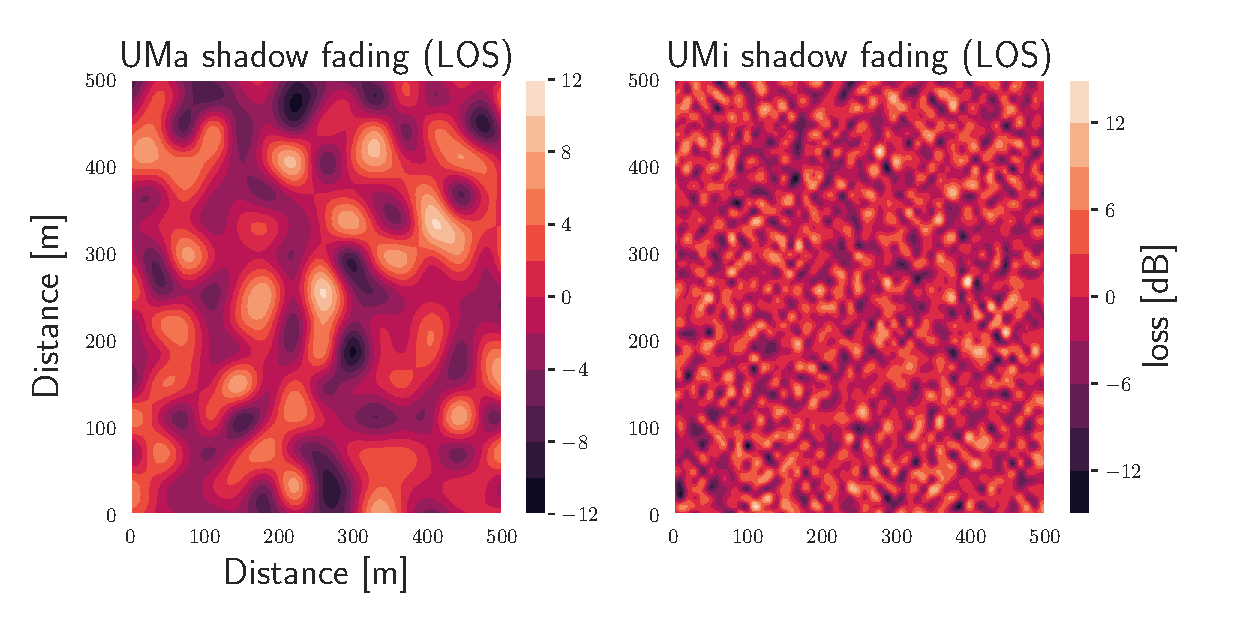
\includegraphics{chapters/part_pathloss/figures/UMaUMiShadowFadingMapLOS.eps}
    \caption{Example of shadowing fading magnitude maps in x,y coordinates with spatial consistency for \gls{uma} and \gls{umi}.}
    \label{fig:uma_umi_shadow_fading_example}
\end{figure}

    
As noted eariler, large-scale and more specifically shadow fading is well represented by a log-normal distribution. Thus $X_\sigma \sim \mathcal{N}(\mu, \sigma^2)$ is a log-normal distribution with mean zero and a variance determined by $\sigma$. The magnitude of $\sigma$ is dependent on the propagation scenario, for instance \gls{uma} or \gls{rma}. The variance of the distribution dictates the variability of the shadowing impairments and is also known as \emph{local variability} \cite{Perez-Fontan2008}. The magnitude of shadowing is determined using measurement studies, such as the one seen in \cite{Sun2016}. The studies mentioned in the fore mentioned work is used as a baseline for the models proposed and defined in \textit{\gls{3gpp} 38.901}. An example of the standard deviation, i.e. the magnitude of shadowing in dB can be observed in Table \ref{tab:sigma_SF} for each of the defined propagation scenarios.


\begin{table}[b]
    \centering
    \begin{tabular}{@{}ll@{}}
    \toprule
    Scenario   & Shadow fading std (dB)               \\ \midrule
    RMa (LOS)  & $\sigma_{SF} = 4$, $\sigma_{SF} = 6$ \\
    RMa (NLOS) & $\sigma_{SF} = 8$                    \\
    UMa (LOS)  & $\sigma_{SF} = 4$                    \\
    UMa (NLOS) & $\sigma_{SF} = 6$                    \\
    UMi (LOS)  & $\sigma_{SF} = 4$                    \\
    UMi (NLOS) & $\sigma_{SF} = 7.82$                 \\ \bottomrule
    \end{tabular}
    \caption{Shadow fading magnitude from \cite{3GPP38901}}\label{tab:sigma_SF}
\end{table}


However, it is also important to note that such distributions have a so-called \emph{decorrelation distance}. This is to ensure spatial consistency between the magnitude of shadowing effects. In other words, obstacles causing the shadowing are likely spatially dependent and thus users moving with a region of the propagation space will experience the same magnitude of shadowing. This is also illustrated in Fig. \ref{fig:shadowing_decorrelation_distance}. The magnitude of shadow fading can be seen as a Gaussian distribution around the mean estimated path loss. The \emph{decorrelation distance} is then the distance between each Gaussian distribution. In practice this can be seen as the shadow fading effects not being sudden, but rather a function of objects surrounding the receiving antenna. If the receiving antenna is to move slowly the shadow fading does not change immediately but related to the so called decorrelation distance. In other words, the decorrelation distance is a term to seperate the objects in the environment that cause and create the shadowing effect. Shadowing a complex function of interactions but it has been found that utilizing such a decorrelation distance is a good approximation. However, it is important to consider also spatial consistency when modelling these impairments


\begin{figure*}[h]
    \centering
    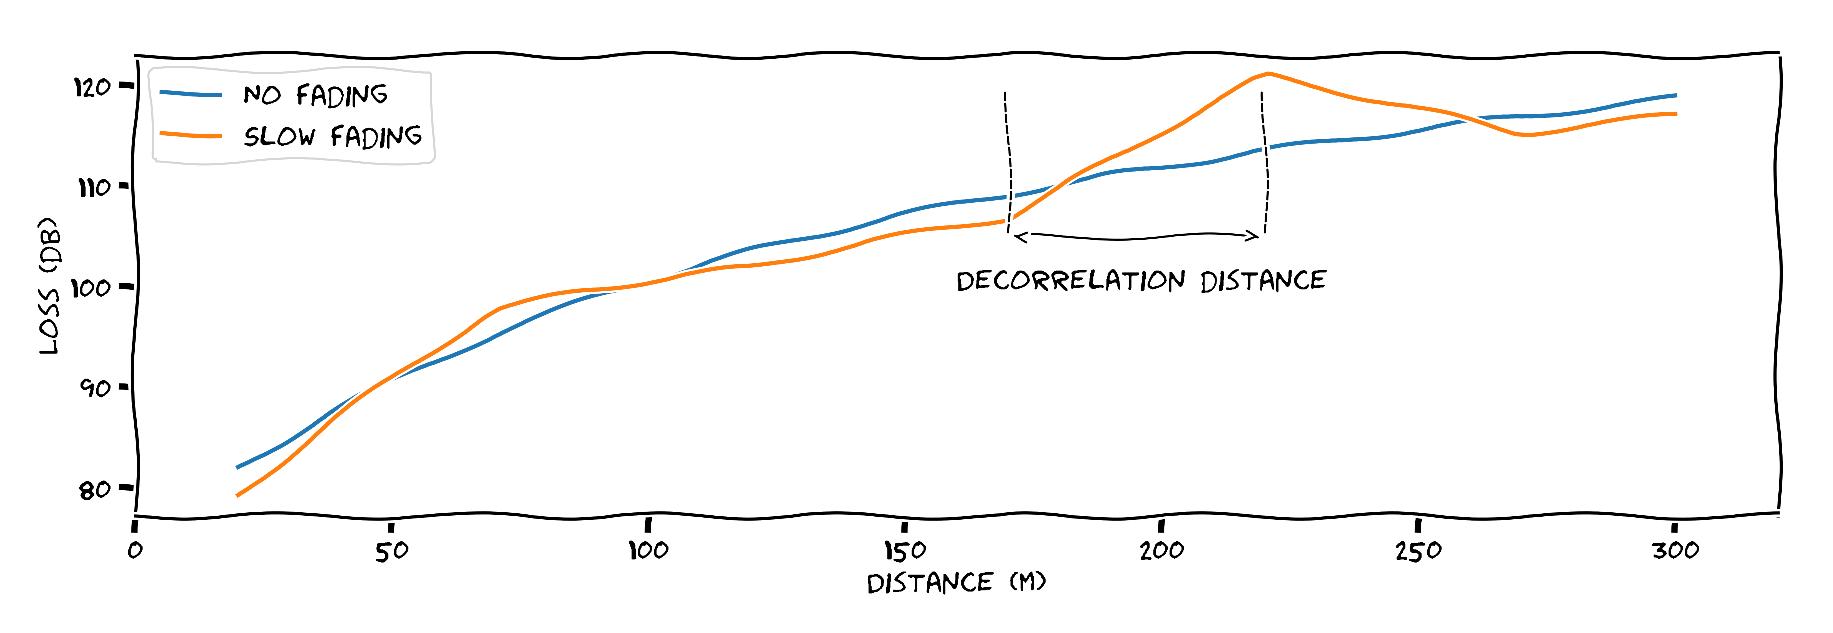
\includegraphics{chapters/part_pathloss/figures/slowfading.eps}
    \caption{Large scale fading, also known as slow fading is the effect of obstacles shadowing the signal. When a receiver moves  the magnitude of such fades change. The distance at which the magnitude changes can be described as a \emph{decorrelation distance}.}
    \label{fig:shadowing_decorrelation_distance}
\end{figure*}



\paragraph{Spatial consistency}
Positions close to one another share common propagation properties, thus it is reasonable to assume that fading impairments have some decorrelation distance. However, in a radio environment this distance needs to also consider a directionality. What this means is that shadow fading is not only dependent on a distance between the fading phenomena but rather dependening on a position with the radio environment. In short, the modelling of shadow fading should consider positions within a space rather than a single distance metric. This results in a necessary translation to 2D coordinates. An example of such a constructed map of shadow fading can be seen in Fig. \ref{fig:uma_umi_shadow_fading_example}.


The figure is produced utilizing a simple procedure as follows 1) realised Gaussian distributions for $N$ points in the grid with a decorrelation distance, and 2) a 2D filtering technique to interpolate values between the realised Gaussian distributions. The number of normal distributions to realise in a position grid is thus given by limits in the X and Y axis and the resulting decorrelation distance. Meaning, for each distance in x and y space, a Gaussian distribution is realised. This results in an incomplete and sparse map which is then 2D filtered.

The large-scale parameters is not only the consideration of shadow fading. More exists with seperate decorrelation distances, meaning the 2D map turns into a multidimensional map of realised distributions. This is computionally infeasible using standard 2D filtering techniques. Using a set of matrix factorization techniques such as the Cholesky factorization the map can be computed while limiting the memory usage and keeping the computational complexity low.


\subsection{Small-scale fading}
\begin{figure}
    \centering
    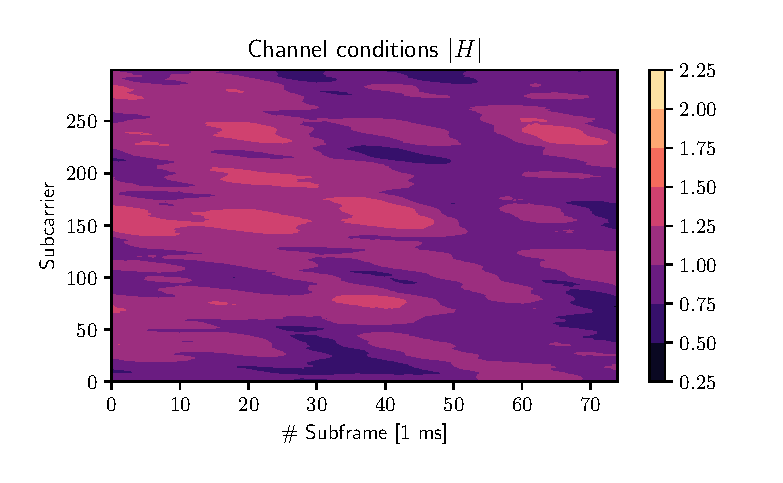
\includegraphics{chapters/part_pathloss/figures/fast_fading_example.eps}
    \caption{Example of the \texttt{\gls{tdl}-E} model at $6$ GHz for $300$ subcarriers.} 
    \label{fig:fast_fading_example}
\end{figure}


The modelling of small-scale fading (or \emph{fast} fading) is more relevant for the immediate design of reliable and efficient communication links. More specifically, fast fading margins is something that is commonly added to link budgets, but, due to the fast varying nature of it; mobile communication systems are unlikely provisioned with respect to this margin. It is something to be considered, but not something that determines cell-site locations and solutions for coverage holes. Here large-scale fading is more relevant. Regardless, the modelling of small-scale fading is paramount to the development of efficient \gls{mimo} solutions and the timing constrained subsystems of mobile communication systems. Common distributions for modelling these impairments include, Rayleigh and Rician.

Since the documents from both \gls{3gpp} and \gls{itu} offer also geometric stochastic models, the modelling of fast fading impairments can be done in several ways. For non-\gls{mimo} study scenarios two models are found in the 38.901 document. More specifically, a so-called \gls{cdl} and \gls{tdl}. A \gls{tdl} model is a common and efficient way of implementing the cause of fast fading i.e. the multi-paths of the channel. The general notion is the implementation of multiple so-called flat-fading generators that are independent. Flat-fading meaning they are not frequency dependent. The implementation is done as a \gls{fir} filter with specific number of taps, each of which have a specific delay (in time),  power attenuation (in dB) and Doppler information. Table 7.7.2-1 in \cite{3GPP38901} describes the delay profile for the so-called \gls{tdl}-A model. The \gls{cdl} model is an extension of the \gls{tdl} model that considers reduced variability and fixed parameters \cite{ITU2412}. An example of the absolute channel coefficients using the \gls{tdl}-E model can be seen in Fig. \ref{fig:fast_fading_example} over time and frequency. 


% Example maybe?

\subsection{Line-Of-Sight}\label{subsec:los}
From the path loss models, e.g. Eq. (\ref{eq:uma_nlos_pathloss_max}) it can be noted that \gls{los} and \gls{nlos} states exists. Determining \gls{los} can be a tricky endavour in outdoor propagation scenarios situations for mobile communication systems. Therefor, the \gls{los} can be modeled in a stochastic manner, using a probability distribution that can be approximated by distance from the transmitter and the height of both the receiver and transmitter antenna. An example of \gls{los} probability can be seen in Fig. \ref{fig:los_probability}. It shows that distances within $20$ meters have $100\%$ of being within \gls{los}, and decreases exponentially given the distance to the transmitter. 

\begin{marginfigure}
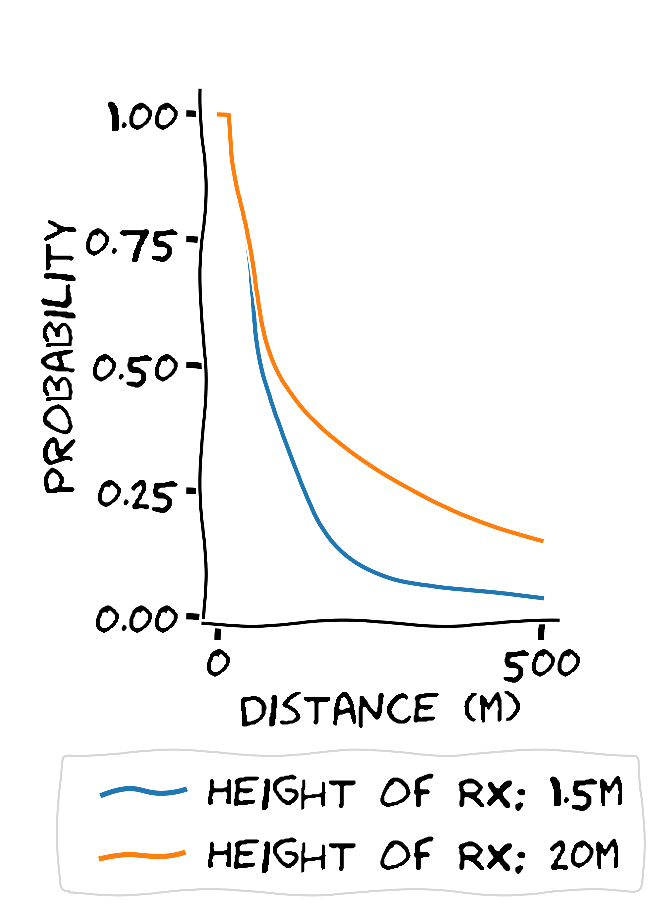
\includegraphics[]{chapters/part_pathloss/figures/LOS_probability.eps}
\caption{The probability of having line-of-sight for a given distance. Two scenarios of receiver height are shown. The probability of having \gls{los} within 25 meters is according to most models 1. }\label{fig:los_probability}
\end{marginfigure}



\subsection{Summary}

The features and details of the channel models described in 3GPP TR 38.901 and ITU-R M.2412 are extensive. Which is a definite need given the board range of supported frequencies (0-100 GHz). A brief view into the documents have been given in this section. It is found that both the documents contain empirical models for a series of different propagation scenarios. The empirical models are based on simple features that can be engineered without the need for complex geographical data. The empirical models are aided by stochastic methods for generating distributions of the most important impairments imposed by wireless transmission. Additionally the modelling approaches are fast and efficient making them useful for approximate predictions of path loss. Furthermore, both the documents contain useful guidelines for creating accurate stochastic channel models. 




\section{Ray-tracing}\label{sec:ray-tracing}

Ray-tracing models consider the physical presence of objects in the propagation model. Depending on the wavelength and the dielectric properties of the objects, the properties of the reflecting, diffracted or absorbed radio waves change. Ray-tracing is a useful tool for many applications, not only mobile communication systems, where the study of particles and their behaviour is to be studied. The recent advanced in computational resources (for instance by using \gls{gpu}) have enabled many advances in the area of ray-tracing technology.

In essence, ray-tracing is a propagation modelling tool that offers estimates, of not only path loss but also the angle of arrival, and the associated time delays. Computing these estimations is enabled by introducing the concept of \emph{rays} that have simplified properties of propagation compared to actual electromagnetic waves. This assumption has shown to be effective at approximating the essential characteristics of electromagnetic propagation. For instance, a ray travels in a straight line if the medium is homogeneous. Furthermore, it obeys the laws of refraction, reflection and diffraction and carries a set of energy \cite{Yun2015}. 
The principle of ray tracing is considering a single point source from which many rays are emanating, also termed \emph{ray-launching}, an example can be seen in Fig. \ref{fig:raytracing_launching}. The multitude of launched rays can then be grouped into different types depending on the interactions occurring in the propagation environment. Some rays are directly \acrlong{los} to the receiving point, causing them to be direct rays. Objects (depending on the material) reflect rays, and some are diffracted. Diffraction causes a single ray to produce a multitude of rays. The combination of these effects and the simplification of using the definition of \emph{rays} can effectively approximate the famous Maxwell equations.  Several algorithms for computing the behaviour of rays can be found in \cite{Yun2015} and references herein.


\begin{figure*}
    \centering
    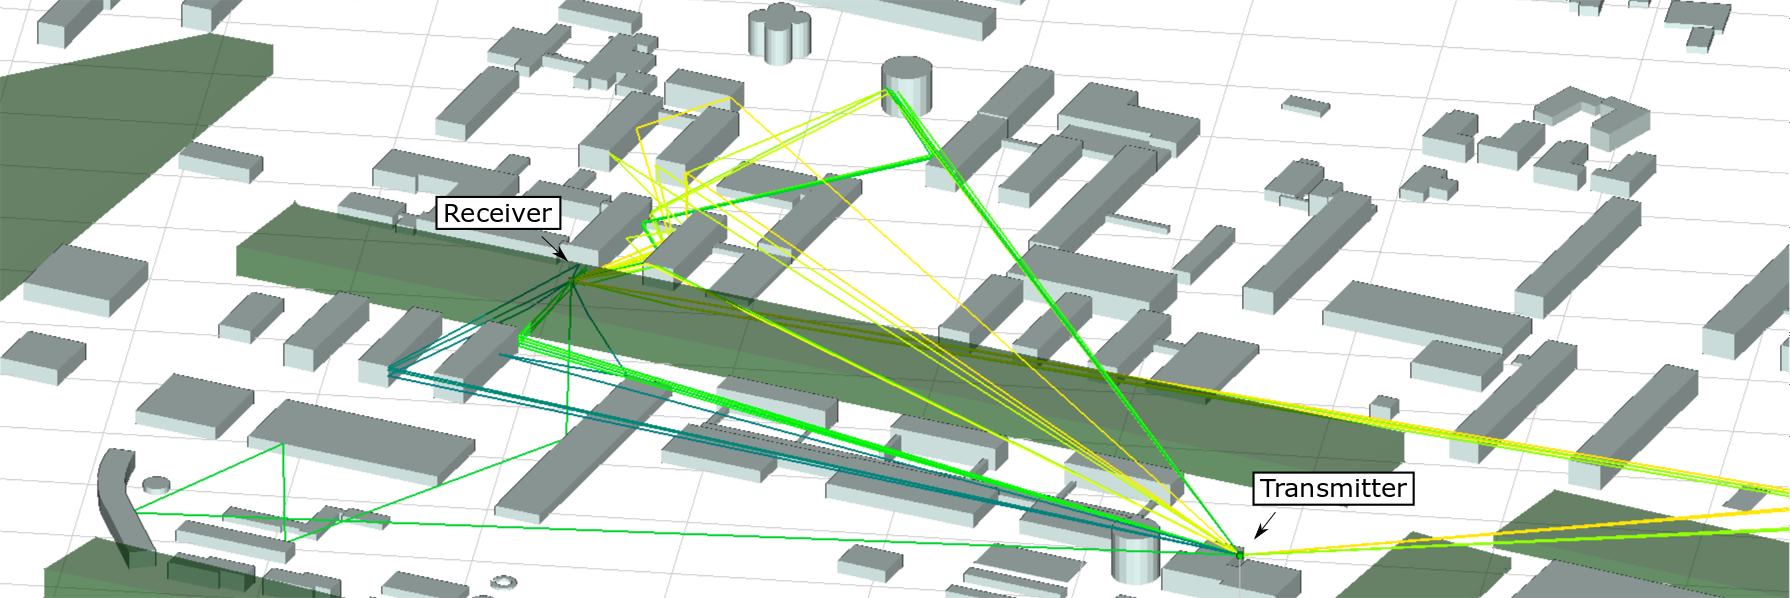
\includegraphics{chapters/part_pathloss/figures/RemcomRayLaunchingv2.png}
    \caption{An example of launched rays in Remcom Wireless Insite}
    \label{fig:raytracing_launching}
\end{figure*}

In outdoor propagation scenarios of mobile communication systems the number of objects significantly vary from region to region. And furthermore, the number of relevant objects change significantly given the change in frequency and thus the wavelength. We use the term \emph{objects} here to represent any obstacle or \emph{thing} in the radio environment. This is for instance, buildings, vegetation, cars and even humans. By having detailed information on all objects in the propagation scenario ray-tracing solutions can be applied and the resulting propagation statistics of the \emph{rays} can be determined. However, it is also clear the such models are data exhaustive and increasingly so as the wavelength shortens \cite{Tse2005FundamentalsCommunication}. Thus for the multitude of high frequencies in the heterogeneous network architecture ray-tracing is simply unfeasible and challenging to approach. But, if the data is available the accuracy is in theory as close to the actual physical interactions as possible.

The data required for modern ray-tracing applied for use in mobile Communication systems can be split into several categories as below
\begin{itemize}
    \item Clutter (vegetation information).
    \begin{itemize}
        \item Position
        \item Height and type.
    \end{itemize}
    \item Buildings.
    \begin{itemize}
        \item Position
        \item Material composition
        \item Height and shape
    \end{itemize}
    \item Terrain. 
    \begin{itemize}
        \item Material composition
        \item Height
    \end{itemize}
\end{itemize}

The data only increases as a multitude of propagation scenarios are considered. For instance, in order to model \gls{o2i} propagation significant detail of not only the buildings and their material is required but also the internal layout and floor dimensions. In addition to these parameters, several configuration elements are also required. Such as the configuration of the transmitter and receiver antennas, along with calibrated noise figures representative of the hardware used. Modern ray-tracing engines such as Remcom Wireless Insite \cite{remcom} simplifies the procedure of integrating a large selection of data by having predefined material composition definitions with permittivity properties. However, not supplied by such modern engines is the data pipeline required for constructing the scene for modelling the propagation scenario. A contribution of this dissertation is the development of a $3$D ray-tracing model of Technical University of Denmark Campus. The necessary details and the resulting procedure for constructing such a model is outline for the remainder of this section

\subsection{$3$D modelling}

The terrain information can in most cases be obtained using survey data, which is in most cases a necessary practice for many applications such as construction, utility and others. The Danish governmental institution \emph{styrelsen for dataforsyning og effektivisering} have made such data public and can be downloaded for free \cite{kortforsyningen}. Furthermore, the entire country of Denmark is \gls{lidar} scanned with high frequency (every 5-10 years) and high resolution. Such a public data set is paramount to obtaining the ray-tracing model as developed for this dissertation. More specifically \gls{lidar} data is supplied with a resolution of 4.5 measurements per $m^2$. An example of such data be seen in Fig. \ref{fig:lidar_data_example}. 

\begin{figure}
    \centering
    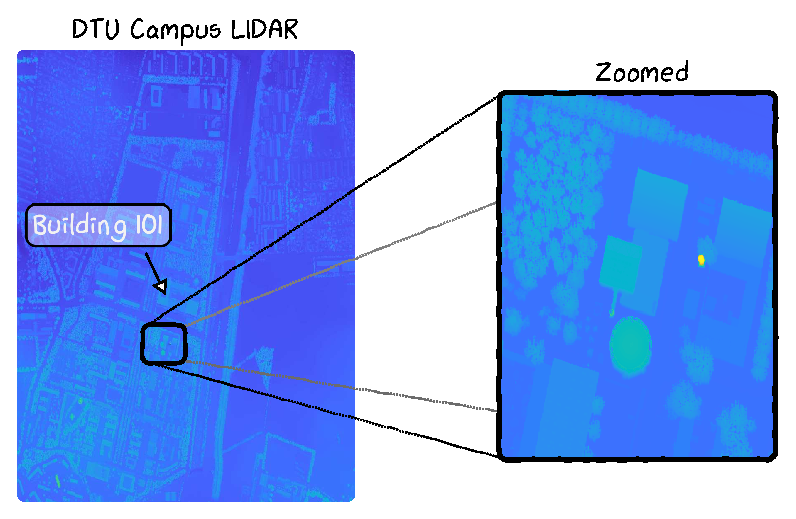
\includegraphics[width=\textwidth]{chapters/part_pathloss/figures/LIDAR_example.eps}
    \caption{Height measurements provided by \cite{kortforsyningen} using a LIDAR scan. Shown is DTU campus with a zoomed cutout. 4.5 points are available per $m^2$. Such data offer the basis for constructing a realistic 3D model for ray-tracing.}
    \label{fig:lidar_data_example}
\end{figure}

Even with this data, a significant effort is required to convert it to independent height of buildings. The procedure is three-fold. Firstly, it requires knowledge of building locations and their respective shapes. Secondly, assumptions of roofing and height must be applied for each building. Third, and lastly, the effective height of the buildings must be extracted. This was performed by utilizing the \gls{lidar} scans to effectively sample the height of buildings. The buildings were identified using zonal descriptions obtained through \gls{osm} \cite{OpenstreetMapWiki}. The mean of all samples within each building footprint (polygons) effectively provided an altitude measurement for each building, and thus a 3D polygon.

The exported file contains polygons, thus buildings and their shape with coordinates and the effective height of each polygon. The effective height is computed as the mean of $N$ number of \gls{lidar} measurements within the building footprints. Thus, if a roof is not flat a significant error to the building height is obtained. Thankfully, most buildings at DTU campus (if not all) have flat roofing. The file can be directly imported into Remcom Wireless Insite where further modelling of antennas are required. Additionally, and possibly even more import, is the definition of materials - this is where the model starts to become increasingly complex. A detailed description of the ray-tracing model can be found in Appendix \ref{app:ray_tracing_model}.

The authors in \cite{Vitucci2015} outline the difficulties of complex ray-tracing models, and more so, the resulting prediction accuracy. There exist a significant lack of literature comparing ray-tracing models and simple empirical models to experimental measurements. Even though the authors in \cite{Vitucci2015} argue the inaccuracy of ray-tracing models - it is still expected that a 3D model of the propagation scenario outperforms any empirical models due to the incorporation of propagation specific information. A result of such a study can be seen in the published work: \cite{Thrane2019ComparisonGHz}. The work compares the resulting 3D ray-tracing model with state-of-the-art empirical as detailed prior in this.



\section{Evaluation of classic methods}\label{sec:comparison_ghz_paper}
The result of a comparison study can be found in the published work \cite{Thrane2019ComparisonGHz}. Two operating frequencies are studied, specifically 811 MHz and 2630 MHz. The study compares existing methodologies such as ray-tracing (see section \ref{sec:ray-tracing}) and empirical models (see section \ref{sec:empirical_path_loss}) for predicting signal quality metrics of \gls{rsrp}. The study is based on experimental drive test data, more information can be found in Appendix \ref{app:drive_test_study_2017}. The measured \gls{rsrp} operates at a bandwidth of $20$ MHz. The base station location is kept constant, therefore the \gls{rsrp} is measured for a single base station with multiple sectors of different operating frequencies. 


\subsection{Results}

\begin{figure*}[thbp]
    \centering
    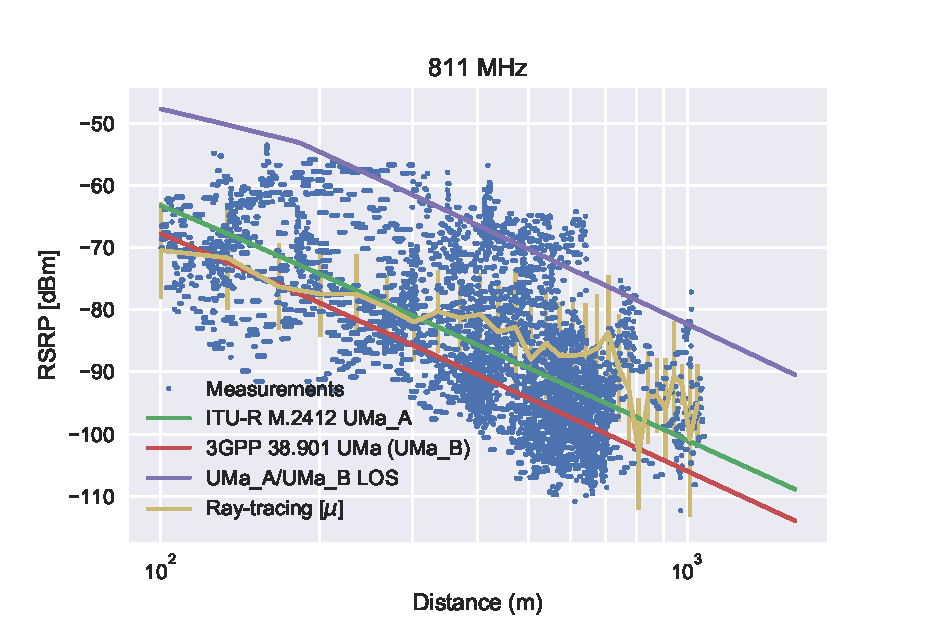
\includegraphics[width=0.48\textwidth]{chapters/part_pathloss/figures/results/811MHz_RSRP.eps}
    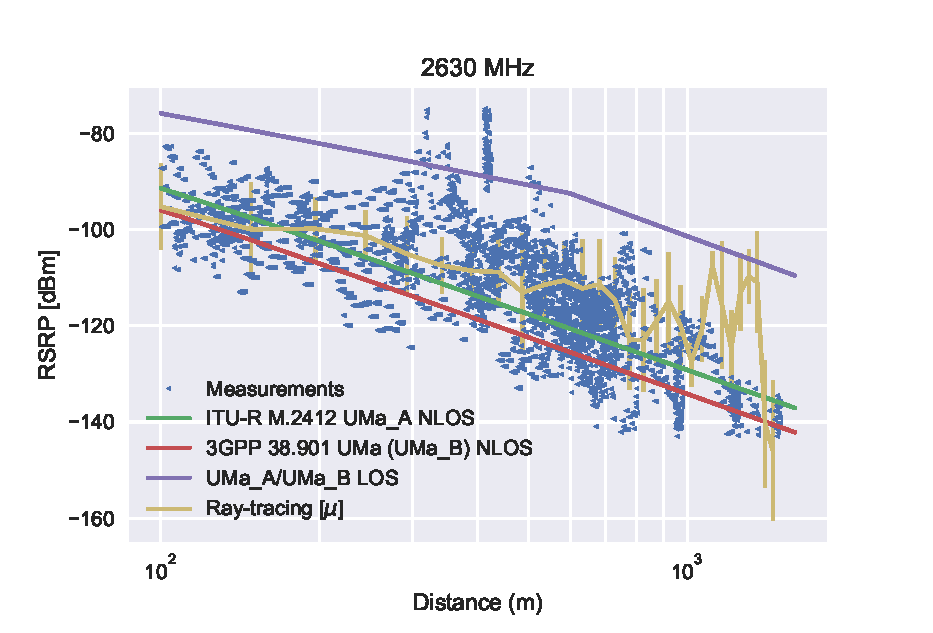
\includegraphics[width=0.48\textwidth]{chapters/part_pathloss/figures/results/2630MHz_RSRP.eps}
    % \vspace{1em}
    % \stepcounter{figure}\label{fig:rsrp_811_2630_distance}
    % \begin{flushleft}
    % \smallskip\noindent\footnotesize Figure \thefigure: The linear regression properties in the log-scale offered by 38.901 (thus \gls{uma}\_B) and ITU-R M.2412 (\gls{uma}\_A) for 811 and 2630 MHz. 
    % \end{flushleft}
    \caption{The linear regression properties in the log-scale offered by 38.901 (thus \gls{uma}\_B) and ITU-R M.2412 (\gls{uma}\_A) for 811 and 2630 MHz.}\label{fig:rsrp_811_2630_distance}
\end{figure*}

Measured \gls{rsrp} for 811 and 2630 MHz respectively can be seen in Fig. \ref{fig:rsrp_811_2630_distance}. The \gls{rsrp} predictions provided by both models, i.e. the ray-tracing and the empirical models are shown. The empirical models of \gls{3gpp} are utilized and termed \uma{B}. The empirical models provided by \gls{itu} M.2412 is denoted \uma{A}. Additional information can be found in section \ref{sec:empirical_path_loss}. The \gls{los} version of both empirical models are identical and shown for reference. 

The ray-tracing model offers point simulations. This is achieved by importing the drive test data into the ray-tracing environment. however, this results in no regression type comparative figure like the empirical models. The binned mean for each distance is shown for reference. A total of 30 bins are used for the averaging. The standard deviation is shown as errorbars. 

It can be seen from the results, that the binned average performance of the ray-tracing model is sufficient for lower distances. This can be seen by the average predicted \gls{rsrp} being more representative of the average \gls{rsrp} measured over the antenna distance separation. Additionally, a few \gls{los} clusters are observed which are well represented by the predictions of the empirical models. 



\begin{figure}
    \centering
    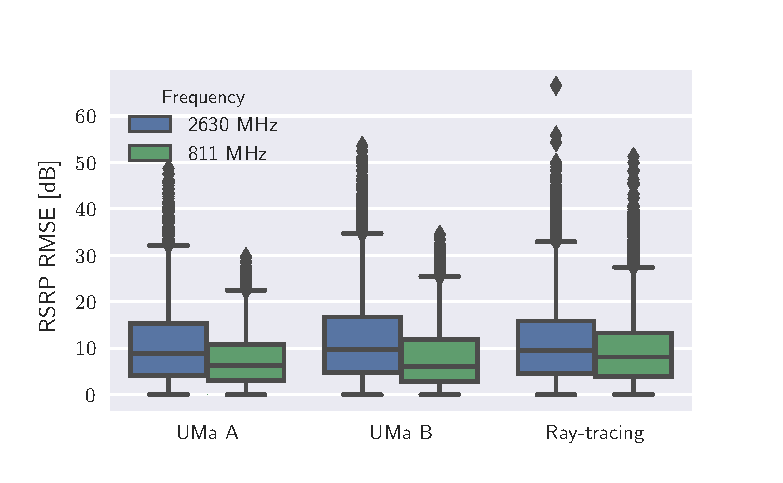
\includegraphics{chapters/part_pathloss/figures/results/improved_boxplot_results_comparison_ghz.eps}
    \caption{Predictive error of ray-tracing model for \gls{rsrp} at 811 and 2630 MHz compared to empirical models \uma{A} and \uma{B}}
    \label{fig:rmse_boxplot_rsrp_comparison}
\end{figure}


The \gls{rmse} (See Eq. \ref{eq:rmse}) is used for evaluating the predictive performance of the empirical and ray-tracing methods. The results can be seen in Fig. \ref{fig:rmse_boxplot_rsrp_comparison}. The best performing model have the lowest \gls{rmse}. The best model is found to be \uma{A} with a \gls{rmse} of $7.6$ dB and $10.76$ dB at $811$ and $2630$ MHz respectively. The ray-tracing model is reported with an \gls{rmse} of $9.25$ dB and $11.13$ dB at $811$ and $2630$ MHz respectively. It can be observed that the performance of the \uma{A} model and the ray-tracing model at 2630 MHz is similar. Finally, it can be seen that on average an improvement in predictive performance of $\approx 3$ dB is achieved on $811$ MHz compared to that of $2630$ MHz.


% \begin{figure*}
%     \centering
%     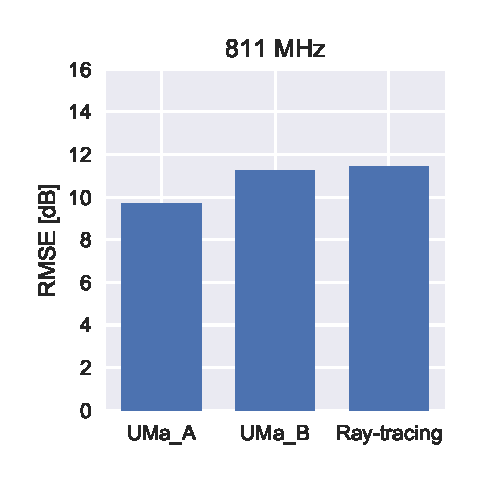
\includegraphics[width=0.48\textwidth]{chapters/part_pathloss/figures/results/811MHz_RMSE.eps}
%     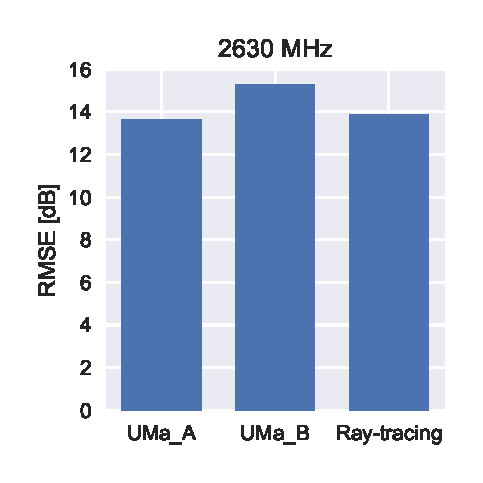
\includegraphics[width=0.48\textwidth]{chapters/part_pathloss/figures/results/2630MHz_RMSE.eps}
%     \vspace{1em}
%     \stepcounter{figure}
%     \begin{flushleft}
%     \smallskip\noindent\footnotesize Figure \thefigure: Error of the empirical path loss models and the ray-tracing model for 811 and 2630 MHz respectively.
%     \label{fig:rsrp_811_2630_RMSE}
%     \end{flushleft}
% \end{figure*}

\subsection{Discussion}
As indicated by the results, and as discussed in the paper \cite{Thrane2019ComparisonGHz}, the results are interesting for one primary reason. The ray-tracing model was expected to outperform the empirical models by some margin. This however, is not the case as the empirical \uma{A} model offers a predictive improvement in \gls{rmse} of $1.65$ dB at 811 MHz, and $0.37$ dB at 2630 MHz for \gls{rsrp}. This is contributed to several reasons, also found in existing literature \cite{Vitucci2015}. While the proposed ray-tracing model may seem complex the results show that it is not complex enough to accurately depict the realistic propagation setting of the measured area. This is identified to be caused by the following short-comings of the proposed ray-tracing model.

\begin{itemize}
    \item Clutter data in the ray-tracing model kept at a minimum.
    \item Approximation and generalization of building materials across architecture. 
    \item Concrete/brick materials assumed with a fixed and constant permittivity.
    \item Significant yearly difference between measurement study area and the LIDAR scan used for generating 3D objects.
    \item Inaccurate modelling of transmitting and receiving antennas
\end{itemize}

Additionally, the results show an overall decrease in predictive performance for all compared models at higher frequencies of $2630$ MHz. The results are inconclusive as to the reasons of this, but it is suspected that the increased frequency and thus lower wavelength increase the influence of smaller objects in the propagation scenario. These objects are not modeled by either the ray-tracing model or the empirical model.

\subsection{Conclusion}
The comparative study shows that current empirical path loss models for \gls{rsrp} predictions are capable of offering satisfactory performance in terms of $7.6$ dB and $10.76$ dB at $811$ and $2630$ MHz respectively. The measurements are furthermore compared to a ray-tracing model of the measured area. The initial hypothesis was that such a model would offer improved prediction performance compared to simple empirical models. This however is not the case, and a decrease in predictive performance is observed for a ray-tracing model, especially at $811$ MHz. Finally, it is found that predictions at $811$ MHz are on average $3$ dB improved to that at $2630$ MHz. 



\section{Summary}
This chapter have briefly introduced the area of wireless propagation modeling. Different models approaches have been introduced and the a comparative performance study have been presented and discussed. The scope of this chapter is reduced to \emph{empirical}- and \emph{ray-tracing}-based wireless channel models as they represent two inherently different means for computing the wireless channel propagation effects. An introduction to state-of-the-art empirical models as provided by \gls{3gpp} have been presented, along with an implementation of a ray-tracing model centered around the campus of the Technical University of Denmark. The differences between the models have been studied, both in terms of performance but also data complexity. The performance of both approaches were further studied by using measurements from a comprehensive drive test. The results showed that the ray-tracing models did not offer any performance gains compared to simple empirical models utilizing simple distance metrics. From theory it is clear that an increased amount of detail of the propagation area will result in more accurate computation of far-field statistics. However, this is not the case with the ray-tracing model implemented. Thus, in practice the increase of data complexity for wireless channel models does not directly translate to improvements in performance. 

While the proposed ray-tracing model suffer from large variability and poor performance several improvements have been identified. For instance, almost no clutter data is imported into the model and the model materials are very approximated. In any case, the empirical models have shown to offer satisfactory performance using simple metrics. Furthermore, the complexity of the model is highly dependent on the application needed. It is thus a constant trade-off between selecting the right model for the task at hand and the data available. Thus it is a challenge to model wireless propagation effects from not only the perspective of improved predictive performance, but also from a data complexity perspective. 

Not only is channel modelling a difficult task, it also impose practical problems of data engineering. It is of great interest to study how adaptive and iterative learned models perform on both performance accuracy but also computational performance. In the next chapter \gls{dl} for path loss estimation is introduced. While the task of current models consist of known model structures and methodologies, by applying \gls{dl} it is desired to learn the optimum model complexity through iterative learning principles as introduced in chapter \ref{ch:mlbasics}. The proposed methodology is shown to be effective in utilizing a completely data-driven approach of obtained measurements, but even more so, by introducing expert knowledge of path loss estimations (as introduced in this chapter) the stability and performance can be improved.